\documentclass[%
a4paper,
12pt,
2.5headlines, 
bigheadings, 
titlepage, 
openbib,
%draft
]{scrartcl}

%%% PACKAGES
\usepackage[ngerman, english]{babel}
%% FONTS


\usepackage[T1]{fontenc}
\usepackage{geometry}
\usepackage[utf8x]{inputenc}
\usepackage{mathpazo}
\usepackage{helvet}
\usepackage{courier}
\usepackage{eurosym}
\usepackage{amsmath}
\usepackage{courier}
\usepackage{scrpage2}
\usepackage{graphicx}
\usepackage{xcolor}
\usepackage{multirow}
\usepackage{varioref}
\usepackage{babelbib}
\usepackage{makeidx}
\usepackage{tabularx}
\usepackage{floatflt}
\usepackage{listings}
\usepackage{color}
\usepackage[pdftex, colorlinks, linktocpage, linkcolor=black, citecolor=black, urlcolor=black]{hyperref}
\usepackage[linesnumbered]{algorithm2e}
\pagestyle{scrheadings}

\definecolor{dkgreen}{rgb}{0,0.6,0}
\definecolor{gray}{rgb}{0.5,0.5,0.5}
\definecolor{mauve}{rgb}{0.58,0,0.82}
\definecolor{code_background}{HTML}{F7F7F7}
\definecolor{code_frame}{HTML}{DDDDDD}
\definecolor{code_comments}{HTML}{969896}
\definecolor{code_keywords}{HTML}{A71D5D}
\definecolor{code_numbers}{HTML}{969896}
\definecolor{code_strings}{HTML}{183691}
\definecolor{code_identifiers}{HTML}{333333}

\lstset{
  language=C++,
    backgroundcolor=\color{code_background},
    commentstyle=\color{code_comments},
    keywordstyle=\color{code_keywords},
    numberstyle=\tiny\color{code_numbers},
    stringstyle=\color{code_strings},
    identifierstyle=\color{code_identifiers},
    basicstyle=\scriptsize,
    aboveskip=5mm,
    belowskip=5mm,
    xleftmargin=0mm,
    xrightmargin=-20mm,
    breakatwhitespace=false,
    breaklines=true,
    captionpos=b,
    keepspaces=true,
    numbers=left,
    numbersep=10pt,
    frameround=ftff,
    frame=single,
    rulecolor=\color{code_frame},
    showspaces=false,
    showstringspaces=false,
    showtabs=false,
    tabsize=2
}

\lstdefinelanguage{JavaScript}{
  keywords={typeof, new, true, false, catch, function, return, null, catch, switch, var, if, in, while, do, else, case, break},
  keywordstyle=\color{blue}\bfseries,
  ndkeywords={class, export, boolean, throw, implements, import, this},
  ndkeywordstyle=\color{darkgray}\bfseries,
  identifierstyle=\color{black},
  sensitive=false,
  comment=[l]{//},
  morecomment=[s]{/*}{*/},
  commentstyle=\color{purple}\ttfamily,
  stringstyle=\color{red}\ttfamily,
  morestring=[b]',
  morestring=[b]"
}


\geometry{a4paper, top=55mm, left=40mm, right=35mm, bottom=40mm,
headsep=10mm, footskip=22mm}
\linespread {1.25}
%%% COMMANDS

	\newcommand{\theauthor}{Tim Oesterreich}
	\newcommand{\matrnr}{770496}
	\newcommand{\thetitle}{\fontsize{18}{16}\selectfont  Racing Line Detection - Recording and Comparison of Racing Lines}
	\newcommand{\thesubtitle}{ Ideallinienerkennung - Aufnahme und Vergleich von Ideallinien}

%%% COLORS
% Rot
\definecolor{hpired}{rgb}{0.686,0,0.204}
% Orange
\definecolor{hpiorange}{rgb}{0.867,0.380,0.031}	
% Gelb
\definecolor{hpiyellow}{rgb}{0.965,0.659,0}			%100 
\colorlet{hpiyellow2}{hpiyellow!60!white}				% 60
\colorlet{hpiyellow3}{hpiyellow!40!white}				% 40
\colorlet{hpiyellow4}{hpiyellow!20!white}				% 20
% Grau
\definecolor{hpigrey}{rgb}{0.376,0.408,0.420}		%100
\colorlet{hpigrey2}{hpigrey!70!white}						% 70
\colorlet{hpigrey3}{hpigrey!50!white}						% 50
\colorlet{hpigrey4}{hpigrey!20!white}						% 20
% Blau
\definecolor{hpiblue}{rgb}{0,0.478,0.620}				%100
\colorlet{hpiblue2}{hpiblue!60!white}						% 60
\colorlet{hpiblue3}{hpiblue!40!white}						% 40
\colorlet{hpiblue4}{hpiblue!15!white}						% 15

%%% OTHER INPUTS
\usepackage{array}
\usepackage{supertabular}
\usepackage{colortbl}

\newcounter{todocounter}
\setcounter{todocounter}{0}
\newcounter{authcounter}
\setcounter{authcounter}{0}
%%% BEGIN Write TODO in File
\def\getdefhelp#1->#2\endhelp{#2}
\def\getdef#1#2{\edef#2{\expandafter\getdefhelp\meaning#1\endhelp}}
\newwrite\TodoDatei
\newwrite\AuthorDatei
\openout\AuthorDatei=author.out
\newcommand{\WriteTodo}[2]{%
	\def\Cont{#2}
	\getdef\Cont\Content
	\edef\WriteIndex{%
		\write\TodoDatei{\string\textcolor{#1}{\string\textbf{\Content}}\string\dotfill\string\pageref{todo:\thetodocounter}}}%
	\WriteIndex}

\newcommand{\WriteAuthor}[1]{%
	\def\Cont{#1}
	\getdef\Cont\Content
	\edef\WriteAuth{\write\AuthorDatei{\Content\string\dotfill\string\ref{auth:\theauthcounter}}}
	\WriteAuth}


%%% END Write TODO in File

% command \BibTeX
\def\BibTeX{{\rm B\kern-.05em{\sc i\kern-.025em b}\kern-.08em
     T\kern-.1667em\lower.7ex\hbox{E}\kern-.125emX}} 

% day in journal: \journalday{date}{titel}{persons}{aktivity}
\newcommand{\journalday}[4]{%
\def\titleTmp{#2}
\subsection*{#1\ifx\titleTmp\empty{}\else{: #2}\fi}
\begin{center}
\begin{tabularx}{\textwidth}{@{}lX@{}}
	Anwesende: & #3\\
	Vorgang: & #4
\end{tabularx}
\end{center}
}

% errorreport: \errorreport{date}{error}{reason}{solution}
\newcommand{\errorreport}[4]{%
\def\dateTmp{#1}
\def\errorTmp{#2}
\def\reasonTmp{#3}
\def\solutionTmp{#4}
\ifx\errorTmp\empty{}\else{%
\subsection*{\ifx\dateTmp\empty{}\else{\hfill(#1)\\}\fi Problem: #2}%
{\begin{center}%
\vskip-1ex%
\begin{tabularx}{\linewidth}{@{}lX@{}}
	Ursache: & \ifx\reasonTmp\empty{unbekannt}\else{#3}\fi\\
	L�sung: & \ifx\solutionTmp\empty{unbekannt}\else{#4}\fi\\
\end{tabularx}%
\end{center}%
}}\fi}

% code: \code[textcolor]{backgroundcolor}{content}
\newcommand{\code}[3][black]{%
	\begin{flushleft}	
		\ttfamily
		\small
		\fcolorbox{#1}{#2}{\textcolor{#1}{\shortstack[l]{#3}}}
	\end{flushleft}
}

% code with white borderline
\newcommand{\codeblank}[3][black]{%
	\begin{flushleft}	
		\ttfamily
		\small
		\fcolorbox{white}{#2}{\textcolor{#1}{\shortstack[l]{#3}}}
	\end{flushleft}
}

% centered code: \centercode[textcolor]{backgroundcolor}{content}
\newcommand{\centercode}[3][black]{%
	\begin{center}	
		\ttfamily
		\small
		\fcolorbox{#1}{#2}{\textcolor{#1}{\shortstack[l]{#3}}}
	\end{center}
}

% centered code with white borderline
\newcommand{\centercodeblank}[3][black]{%
	\begin{center}	
		\ttfamily
		\small
		\fcolorbox{white}{#2}{\textcolor{#1}{\shortstack[l]{#3}}}
	\end{center}
}


% annotation in colored box: \annot[text- and bordercolor]{backgroudcolor}{contents}
\newcommand{\annot}[3][black]{%
	\begin{center}	
		\fcolorbox{#1}{#2}{\textcolor{#1}{\shortstack[l]{\vspace*{1ex}\\\hspace*{.025\textwidth}\textbf{Anmerkung:}\\\hspace*{.05\textwidth}\parbox{.88\textwidth}{#3\vspace*{2ex}}\hspace*{.05\textwidth}}}}
	\end{center}
}

% annotation in colored box: \annot[text- and bordercolor]{backgroudcolor}{contents}
\newcommand{\hint}[3][black]{%
\begin{figure}[!t]
  \centering
  \fcolorbox{#1}{#2}{
    \begin{minipage}{.96\linewidth}
      \hspace*{.025\linewidth}\parbox{.93\linewidth}{\textbf{Hinweis:}}\hspace*{.025\linewidth}\\
      \hspace*{.05\linewidth }\parbox{.88\linewidth}{\vspace*{3ex}#3\vspace*{3ex}}\hspace*{.05\linewidth}
    \end{minipage}
  }
\end{figure}
}

\newcommand{\colorparbox}[3][.985\textwidth]{%
\begin{flushleft}
\fcolorbox{black}{#2}{\parbox{#1}{#3}}
\end{flushleft}
}

\newcounter{versionID}
\newenvironment{versioning}[1][hpiblue4]{%
\setcounter{versionID}{0}
\begin{center}	
	\tablefirsthead{%
		\hline
		\rowcolor{#1}
		\parbox[c][2em][c]{\linewidth}{\centering\textbf{lfd. Nr.}} &
		\parbox[c][2em][c]{\linewidth}{\centering\textbf{Bearbeiter}} & 
		\parbox[c][2em][c]{\linewidth}{\centering\textbf{�nderungen}}\\
		\hline}
	\tablehead{%
		\extrahead
		\hline
		\rowcolor{#1}
		\parbox[c][2em][c]{\linewidth}{\centering\textbf{lfd. Nr.}} &
		\parbox[c][2em][c]{\linewidth}{\centering\textbf{Bearbeiter}} & 
		\parbox[c][2em][c]{\linewidth}{\centering\textbf{�nderungen}}\\
		\hline}
	\tabletail{%
		\hline
		\multicolumn{3}{|r|}{\cellcolor{hpiblue4}\small\sl Fortsetzung auf der n�chsten Seite}\\
		\hline}
	\tablelasttail{}
	\begin{supertabular}{|p{.1\linewidth}|p{.25\linewidth}|p{.5\linewidth}|}
	}{%
	\end{supertabular}
\end{center}
\newwrite\VersionDatei
\openout\VersionDatei=theversion.aux
\write\VersionDatei{\theversionID}
\closeout\VersionDatei
%\vfill
}

\newcommand{\version}[2]{%
\parbox{\linewidth}{\centering\stepcounter{versionID}\theversionID} & 
\parbox[t]{\linewidth}{\centering#1} &
#2 \\\hline
}

\newcommand{\currentversion}[1][]{
\def\test{#1}
\def\drafttest{draft}
\def\finaltest{final}
\ifx\test\drafttest
	\def\versiontext{(Entwurf)}
\else
	\ifx\test\finaltest
		\def\versiontext{(Final)}
	\else
		\def\versiontext{}
	\fi
\fi
\vskip.3cm
\newread\DatenDatei
\openin\DatenDatei=theversion.aux
\ifeof\DatenDatei\def\curVers{---}\else\read\DatenDatei to \curVers\fi
\closein\DatenDatei
{\small Dokumentversion: \curVers{}\versiontext}}

%% Acceptance Criterions
\newenvironment{acceptance}[1][hpiblue4]{%
\begin{center}	
	\tablefirsthead{%
		\hline
		\multicolumn{2}{|l|}{\cellcolor{hpiblue3}\bfseries Abnahmekriterien:}\\
		\hline}
	\tablehead{%
		\hline
		\multicolumn{2}{|l|}{\cellcolor{hpiblue3}\bfseries Abnahmekriterien (Fortsetzung):}\\
		\hline}
	\tabletail{%
		\multicolumn{2}{|r|}{\cellcolor{hpiblue4}\small\sl Fortsetzung auf der n�chsten Seite}\\
		\hline}
	\tablelasttail{}
	\begin{supertabular}{p{.23\linewidth}p{.7\linewidth}}
	}{%
	\end{supertabular}
\end{center}
\vfill
}

\newcommand{\criterion}[3]{%
	& \\
	\rowcolor{hpiblue4}Ausgangssitiation: & #1 \\
	Ereignis: & #2 \\
	Erwartetes Ergebnis: & #3 \\
}

\newcommand{\authindex}[1]{\expandafter\index{#1}}
%% SecAuthor
\newcommand{\secauthor}[2]{%
\def\secChap{chapter}
\def\secSect{section}
\def\secSubs{subsection}
\edef\refer{#1!Abschnitt \thesection}
\def\sec{#2}
\ifx\sec\secChap\edef\refer{#1!Kapitel \thechapter}\fi
\ifx\sec\secSect\edef\refer{#1!Abschnitt \thesection}\fi
\ifx\sec\secSubs\edef\refer{#1!Abschnitt \thesubsection}\fi
\label{auth:\theauthcounter}
\authindex{\refer}
%In Datei schreiben
%\WriteAuthor{#2}
\stepcounter{authcounter}
}

%% Todo
\newcommand{\todo}[2][normal]{%
\def\test{#1}
\def\hightest{high}
\def\lowtest{low}
%\def\normaltest{normal}
\ifx\test\hightest
	\def\prioritycolor{hpired}
\else
	\ifx\test\lowtest
		\def\prioritycolor{hpiyellow}
	\else
		\def\prioritycolor{hpiorange}
	\fi
\fi
\par{\raggedright
	\color{\prioritycolor}TODO: #2
	\label{todo:\thetodocounter}
	\WriteTodo{\prioritycolor}{#2}
	\stepcounter{todocounter}
}\par
}

\newif\ifnotdone

\newcommand{\readLine}[1]{%
\ifeof#1
	\def\tobedone{}
	\notdonefalse
\else
	\read\TodoFileIn to \tobedone
	\notdonetrue
\fi
\tobedone\par}

\newcommand{\listtodo}{%
\begin{flushleft}
	\newread\TodoFileIn
	\openin\TodoFileIn=todo.out
	\loop
		\readLine{\TodoFileIn}
	\ifnotdone
	\repeat
	\closein\TodoFileIn
	\immediate\openout\TodoDatei=todo.out
\end{flushleft}
}

%%% XML-Command
\newdimen\LineFeedDim
\LineFeedDim = 1.5em
\newdimen\LineFeed
\newif\ifXMLintern

\newcommand{\Tag}[4][black]{%
\ifXMLintern\\\hskip\LineFeed\fi%
\XMLinternfalse%
\textcolor{#1}{<#2}%
\def\paratest{#3}%
\ifx\paratest\empty{}%
\else{} #3%
\fi%
\global\advance\LineFeed by \LineFeedDim%
\def\contenttest{#4}%
\ifx\contenttest\empty%
	\global\advance\LineFeed by -\LineFeedDim\textcolor{#1}{/>}%
\else%
\textcolor{#1}{>}\\\hskip\LineFeed#4\\%
\global\advance\LineFeed by -\LineFeedDim\ifdim\LineFeed > 0em\hskip\LineFeed\fi\textcolor{#1}{</#2>}%
\fi\XMLinterntrue%
}

%% <? ... ?> als Argument �bergeben -> processing, comment, normal
\def\proctest{processing}
\def\commtest{comment}
\def\normtest{normal}
\newcommand{\LineTag}[4][normal]{%
\ifXMLintern\\\hskip\LineFeed\fi%
\XMLinternfalse%
\def\argtest{#1}%
<\ifx\argtest\proctest ?\else\ifx\argtest\commtest !-- \fi\fi#2%
\def\partest{#3}%
\ifx\partest\empty%
\else{} %
	#3%
\fi%
\def\contenttest{#4}%
\ifx\contenttest\empty%
\def\argtest{#1}%
\ifx\argtest\proctest{} ?\else\ifx\argtest\commtest{} --\else/\fi\fi>%
\else> #4 </#2>\fi\XMLinterntrue%
}

\newcommand{\EmptyTag}[1][]{%
\ifXMLintern\\\hskip\LineFeed\fi#1\parbox[c][1ex][c]{1ex}{}\XMLinterntrue%
}

\newcommand{\NewLinePar}{%
\\\hskip\LineFeed\hskip3em
}

\newcommand{\xml}[3][black]{%
	\LineFeed=0em
	\XMLinternfalse
	\small
	\fcolorbox{#1}{#2}{\ttfamily\shortstack[l]{#3}}
}

\newcommand{\soapmsg}[7][hpigray4]{%
	{\centering
	\begin{tabularx}{\linewidth}{|l|X|}
		\hline
		\cellcolor{#1}K�rzel & #2 \\
		\hline
		\cellcolor{#1}Consumer & #3 \\
		\hline
		\cellcolor{#1}Request Parameter & #4 \\
		\hline
		\cellcolor{#1}Response Parameter & #5 \\
		\hline
		\cellcolor{#1}Kurzbeschreibung & #6 \\
		\hline%
		\cellcolor{#1}Doppelter Request & #7 \\
		\hline
	\end{tabularx}
	}
}

\newcommand{\myabstract}[2]{%
	\def\germtest{#1}
	\def\engltest{#2}
	\ifx\germtest\empty
		\ifx\engltest\empty
		\else
			\hbox{ }
			\vfill
		\fi
	\else
		%\hbox{ }
		%\vfill
  \fi
	\ifx\germtest\empty\else
  	\begin{quotation}
  	\begin{center}\normalfont\sectfont\nobreak Kurzfassung\end{center}
  	#1
  	\end{quotation}
  	\vskip1cm
  \fi
  \ifx\engltest\empty\else
  	\begin{quotation}
  	\begin{center}\normalfont\sectfont\nobreak Abstract\end{center}
  	#2
  	\end{quotation}
	\fi
	\ifx\germtest\empty
		\ifx\engltest\empty
		\else
  		\vfill
  		\vfill
  		\clearpage
		\fi
	\else
  	\vfill
  	\vfill
  	\clearpage
  \fi
}
% Eigene Umgebungen
\newenvironment{otherenumi}[1]{%
	\renewcommand*{\labelenumi}{#1}
	\begin{enumerate}
	}{%
	\end{enumerate}
	\renewcommand*{\labelenumi}{\alph{enumi})}}
\newenvironment{otherenumii}[1]{%
	\renewcommand*{\labelenumii}{#1}
	\begin{enumerate}
	}{%
	\end{enumerate}
	\renewcommand*{\labelenumi}{\alph{enumi})}}

\newcommand{\frontmatter}{\pagenumbering{roman}}
\newcommand{\mainmatter}{\pagenumbering{arabic}\setcounter{page}{1}}
%%% INCLUDE ONLY
\setlength{\parindent}{0cm}
\setlength{\parskip}{0.25cm}
\graphicspath{{utils/}}
%%% DOCUMENT
\begin{document}
	%%% HEADER AND FOOTTITLES
	%\selectlanguage{ngerman}
	\selectlanguage{english} % {ngerman}
	\automark{section}
	\ohead{
\includegraphics[height=1.3cm,clip,viewport={0 60 250 180}]{utils/hpi_logo.pdf}}
	\chead{}
	\ihead{\headmark}
	\setheadsepline{1.0pt}[\color{hpigrey}]
	%%% TITLEPAGE
	\hypersetup{%
		pdftitle	= {\thetitle},
		pdfsubject	= {Bachelor Thesis},
		pdfauthor	= {\theauthor},
		pdfcreator	= {PDFLaTeX},
		pdfproducer	= {LaTeX with hyperref and thumbpdf}
			   }
	
		\titlehead{
	%\parbox[b]{10cm}{\sffamily{\Large Hasso Plattner Institut}  \\Prof.~Dr.~Helmertstra�e~2-3 \\14482 Potsdam} 
	\centering
	
\includegraphics[height=4cm]{utils/hpi_logo_text.pdf}
	
	}		\subject{{\LARGE Bachelor's Thesis}\\}
	\title{\thetitle}
	\subtitle{\thesubtitle}
	\author{{\small by}\\\textbf{\theauthor}}
	%\dedication{Widmung\\mit mehreren\\Zeilen.}
	\date{Potsdam, June 2016}
	\publishers{
		\textbf{Supervisor}\\
		\vskip1em
		Prof. Dr. Christoph Meinel,\\		
		Philipp Berger, Patrick Hennig\\
	
		\vskip2em
		\textbf{Internet-Technologies and Systems Group}
		}
	\frontmatter
	\maketitle
	%\input{titlepage_german}
		
		
		
		
	\section*{Disclaimer}

I certify that the material contained in this dissertation is my own work and does not contain significant portions of unreferenced or unacknowledged material. I also warrant that the above statement applies to the implementation of the project and all associated documentation.\\\\
Hiermit versichere ich, dass diese Arbeit selbst\"{a}ndig verfasst wurde und dass keine anderen Quellen und Hilfsmittel als die angegebenen benutzt wurden. Diese Aussage trifft auch f\"{u}r alle Implementierungen und Dokumentationen im Rahmen dieses Projektes zu.

	\begin{flushleft}
	Potsdam, \today
	\end{flushleft}
	\begin{picture}(150,70)
		\put(0,15){\line(1,0){150}}
		\put(0,0){(\theauthor)}
	\end{picture}
	\clearpage
	
	%%% Abstract
	\myabstract
	{%
	% deutsche Zusammenfassung
	Im Motorsport dreht sich alles darum so schnell wie möglich um die Rennstrecke zu fahren. Der wichtigste und zugleich am meisten vom Fahrer beeinflusste Schritt dabei ist die Rennlinie, insbesondere das Treffen der Idealllinie in Kurven. Unser Rennanalysesystem sammelt verschiedene fahrzeugbezogene Daten um den Fahrstil eines Rennfahrers zu evaluieren und mit anderen Fahrern zu vergleichen. Dadurch kann dieser einen zeitlichen Vorteil gegenüber seinen Kontrahenten bekommen.

	Diese Arbeit fokussiert sich dabei vor allem auf das Aufnehmen und Vergleichen der Rennlinien mit verschiedenen Methoden, wie Visual Odometry\footnote{eine Video-basierende Bewegungserkennungsmethode} und Fahrbahnranderkennung und das Benutzen dieser Daten zur Analyse des Fahrverhaltens von verschiedenen Fahrern. Wir benutzten dafür eine kamerabasierende Methode, um externe Abhängigkeiten so gering wie möglich zu halten.

	Als Resultat erhielten wir ein System, das eine höher verfügbare und genauere Rennlinienerkennung bereitstellen konnte, als mit einer GPS-basierenden Methode möglich gewesen wäre. Zusätzlich implementierten wir eine einfache, aber effektive Möglichkeit, die erhaltenen Daten so darzustellen, dass Rennfahrer damit ihre Rundenzeiten verbessern können.
	\clearpage
	}{%
	% englischer abstract
	Motor racing is all about getting around a track as fast as possible. One of the most important and most driver-influenced steps in achieving best times is the racing line, especially hitting the ideal racing line through corners. Our race analysis system collects different car-based data to evaluate and compare the driving style of drivers which helps them gain an advantage over the competitors.

	This thesis especially focuses on the recording and comparison of racing lines using different methods, like Visual Odometry\footnote{a camera-based movement detection method} and lane detection and using these extracted data to analyze the driving behavior of different drivers. A camera-based approach is used to minimize external dependencies.

	As a result, we developed a system that could provide a more available and accurate racing line detection than a GPS-based method would be able to achieve. Also a simple, but effective way of displaying the extracted data so that racing drivers are able to improve their lap times.
	}
	
	%%% TOC
	\tableofcontents
	\clearpage
	%%% INCLUDES
	\mainmatter

	%%%%%%%
	%% Add content here !!! %%%
	\section{Introduction}
\label{sec:intro}

\subsection{Motivation}
The trajectory around a track that allows a given vehicle to traverse the circuit in the minimum amount of time is called the ideal racing line. There are a lot of parameters that determine the minimum lap time. In general it is a trade-off between the length of the taken line and the speed carried around the track, which in most cases turns out to be the line with the least curvature.  
Needless to say, in a race this is the path every driver wants to take. In reality, however, this isn't an easy task. In order to achieve best times, a racing driver has to remember exactly which corner of the track comes next, how fast they can take this corner, see how the car is positioned on the track and process much more information.\\
To assist aspiring drivers feel like professionals, we implemented a racing driver analysis system, that is capable of recording, comparing and evaluating race related data. The system saves a complete history of the many sensor data values, like speed, throttle position and safety relevant features, like engine temperature, the car produces. Also it tracks the car on the course using a combination of different methods.
This car tracking will be the main focus of this thesis. \\
The comparison of two drivers requires very robust measurements, that return the same result for every given input.
The most common tracking method, GPS, relies on external sources, namely satellites that communicate with the GPS device. The biggest problem with this traditional approach is that GPS isn't fully available everywhere. Especially on remote areas, which is where most race tracks are, there tends not to be complete coverage. This would result in faulty results and incomparable racing lines.\\
In order to break away from these dependencies, we used a camera-based approach. This allows us to track the relative translation and rotation of the vehicle independent of its speed, location or surroundings.
Apart from the recording of these racing lines, this paper also discusses how to process the obtained data in order to provide a useful support for racing drivers.

\subsection{Project Scope}
During the one year long bachelor project "Feel the Car - Automatic A\-no\-ma\-ly Detection for Unstructured Test Drive Data" at the Hasso-Plattner-Institute in Potsdam, I worked together with four fellow students and in cooperation with Mercedes-AMG on analyzing video and sensor data from car test drives.
Part of the project was to find a possibility to retrospectively evaluate a race for a given driver. This is especially useful for AMGs Driving Academy \footnote{\url{http://www.mercedes-amg.com/driving-academy/}}, which is a service that lets non-professional drivers drive on race tracks and become a racing driver.\\
To achieve this goal, and other requirements, such as detecting potholes on the street or security relevant warning signs in races, we used a stereo camera and a mini-computer that processed the incoming raw data.
Additionally, an On-Board-Diagnostic 2 (OBD-II\footnote{\url{http://www.obdii.com/}}) dongle was used to extract the sensor data that cars have already integrated.
The analyzed result was then displayed in our web application, which also provided a driver profile page that provides a detailed overview of their recorded laps.
\clearpage

\subsection{Problem Context}
\label{sec:context}

\begin{figure}[!ht]
	\centering
	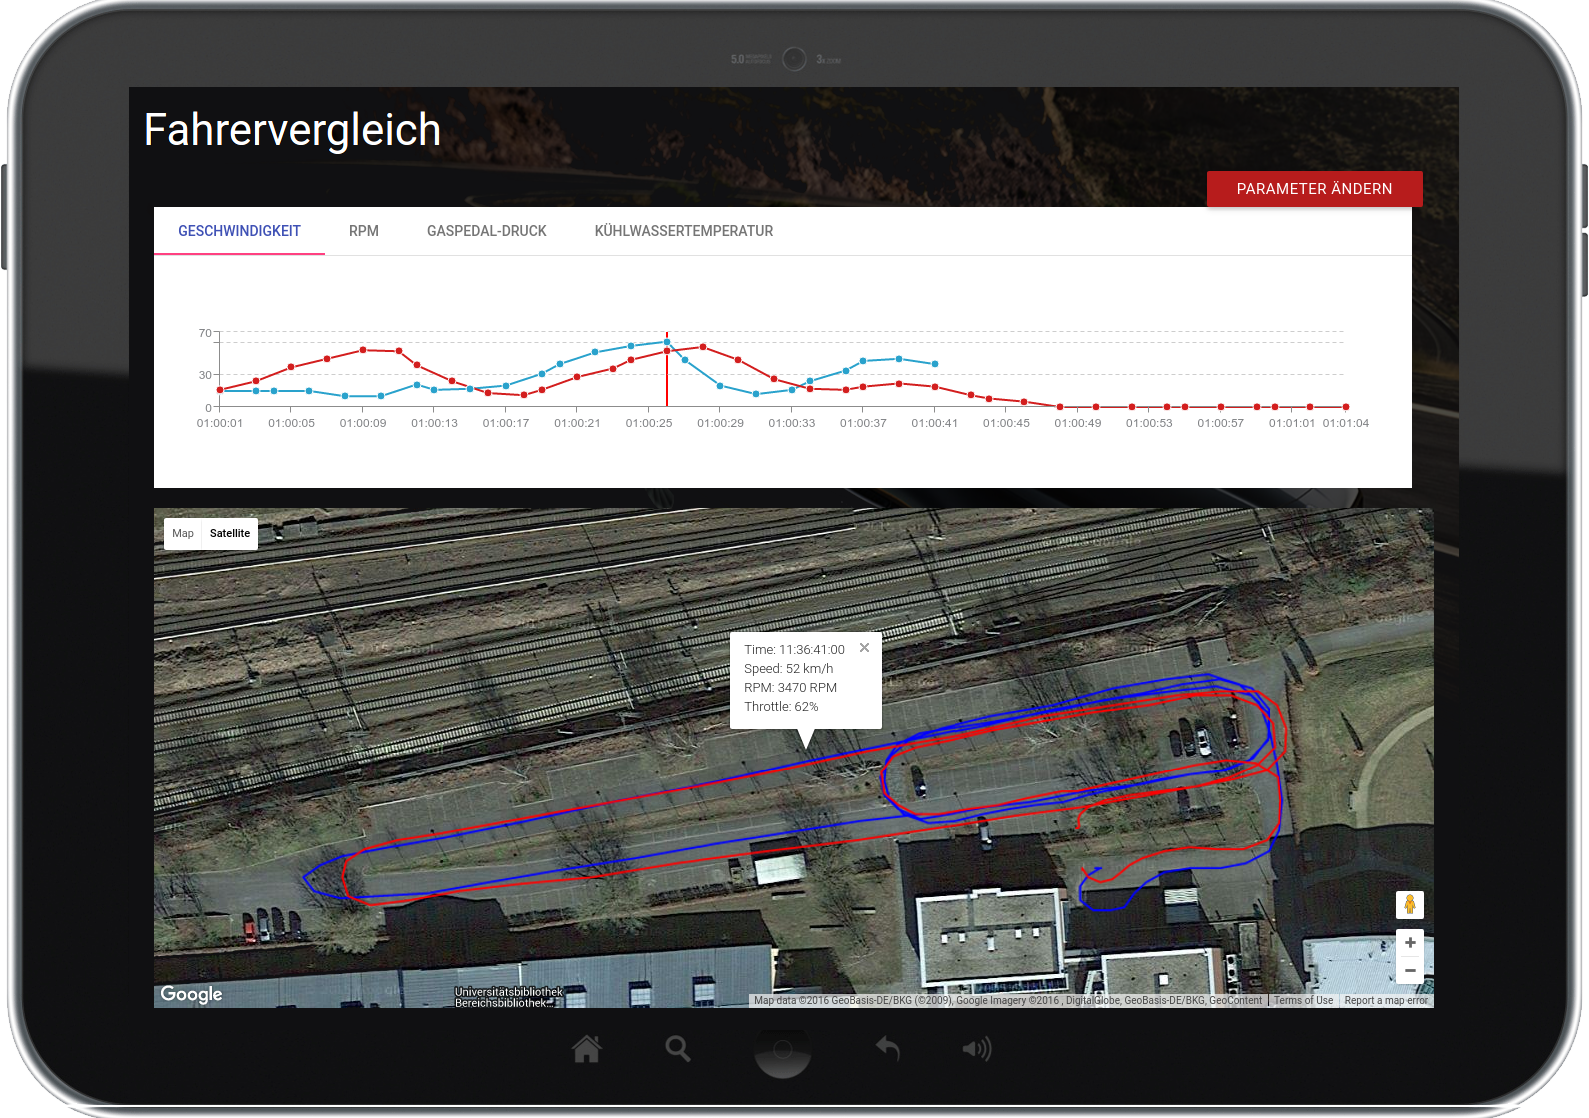
\includegraphics[width=\textwidth]{tablet_with_driver_comparison}
	\caption{Driver Comparison}
	\label{fig:comparison_with_overlay}
\end{figure}

Initially, our task was to analyze existing video material from test drives made by AMG. The exact specifications of this analysis were defined at a meeting with AMG and developed to mainly consist of video- and sensor-based driving aids for drivers at the AMG Driving Academy. Besides the detection of security-relevant events, like warning flags, cars leaving the track into the gravel bed or potholes on the street, we also wanted to find a way to compare and evaluate the driving behavior of two drivers.
During our first tests, which started with a mobile phone camera, we found out that there are a lot of challenges and prerequisites in video analysis. For example, every camera has to be calibrated first, to compute for the individual distortion a camera lens causes. This is not only a fairly complex task that requires high accuracy, it also prevents an easy replacement of camera hardware.\\
This made us look into alternatives and we decided to use a stereo camera. A stereo (or 3D) camera is able to determine metric measurements from the camera image, which enables it to calibrate itself. Also the additional information we can extract from a 3D image made a more accurate and faster detection possible.\\

\begin{figure}[!ht]
		\centering
		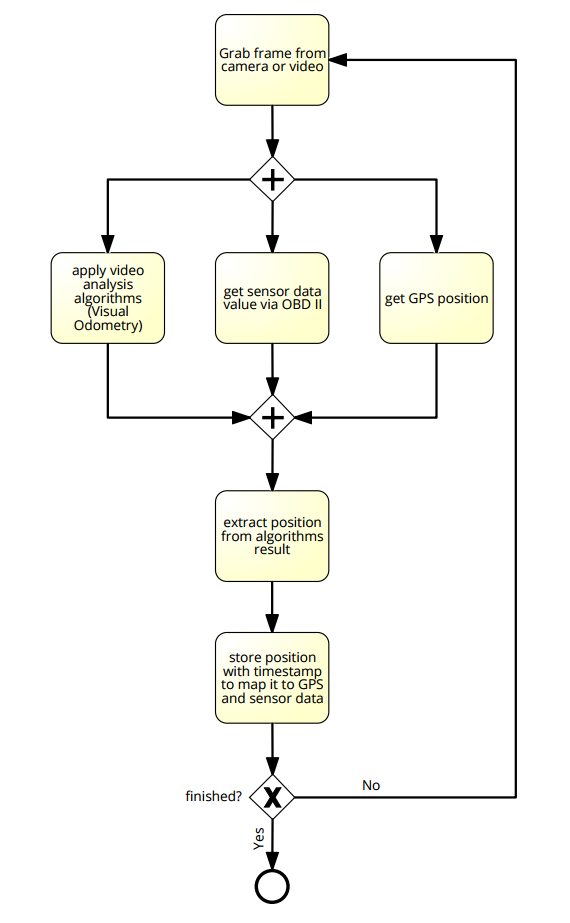
\includegraphics[width=.6\textwidth]{racing_line_recording}
		\caption{Process Diagram Racing Line Recording}
		\label{fig:racing_line_recording}
\end{figure}

Using techniques that will be described in section \ref{sec:algorithm}, we were able to record the racing line of a car based on a stereo video and GPS. Together with the extracted sensor data from the OBD II interface, we stored the points in a database. The process is depicted in Figure \ref{fig:racing_line_recording}.

\begin{figure}[!ht]
	\centering
	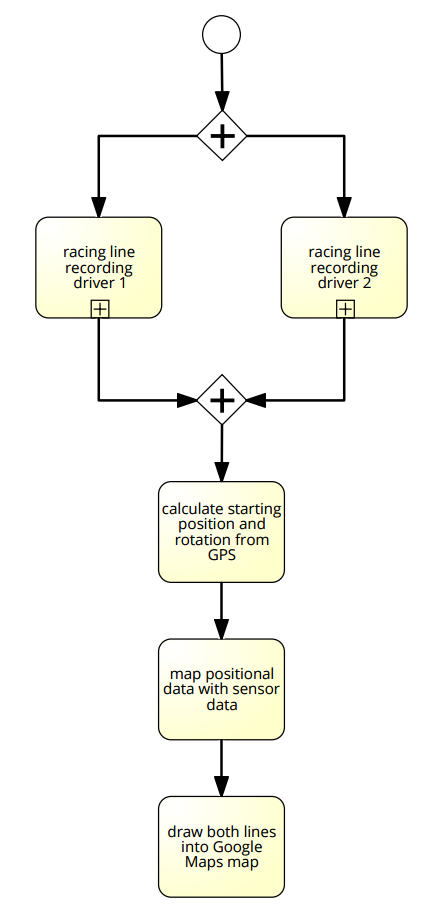
\includegraphics[width=.5\textwidth]{racing_line_comparison}
	\caption{Process Diagram Racing Line Comparison}
	\label{fig:racing_line_comparison}
\end{figure}

Figure \ref{fig:racing_line_comparison} shows how the recorded racing lines can then be compared. We decided to use a Google Maps integration to properly determine where on the track potential improvements can be found. Because of the nature of our recording algorithms, calculating a relative position that can't on itself be mapped to a geographic location, a few preparations, like calculating the starting point and rotation, have to be done. These are further described in Section \ref{sec:comparing}. Interesting data values were displayed by coloring in the racing line in case of the detailed driver view (figure \ref{fig:driver_detail}) or using an info window which gives an overview of the data at a given point (figure \ref{fig:comparison_with_overlay}).

\begin{figure}[!ht]
	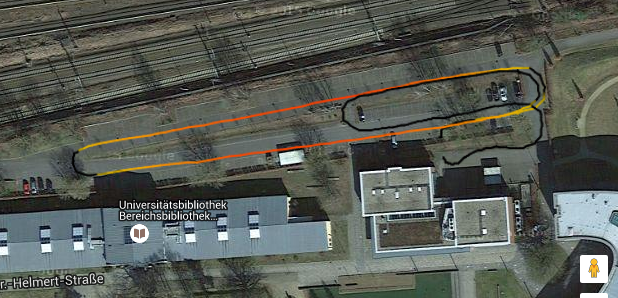
\includegraphics[width=\textwidth]{driver_detail_screenshot}
	\caption{Detailed Driver Overview}
	\label{fig:driver_detail}
\end{figure}

\clearpage
	\section{Related Work}
\label{sec:related_work}

\subsection{Racing Line calculation}
Contrary to most racing sports, where a racing line is usually drawn by an expert, video games, especially from independent developers, tend to concentrate on calculating the racing line for the computer-controlled cars.

\subsubsection{Vamos Racing Simulator}
One example is the \textit{Vamos racing simulator}\footnote{\url{http://vamos.sourceforge.net/}}. It uses an iterative cur\-va\-ture-min\-i\-mi\-za\-tion technique, simulating spring-loaded hinges that are placed in the middle of the track. The lateral forces a car produces during cornering are used to simulate the opening or closing of these hinges, iteratively shaping the racing line. After a certain number of iterations the curve stabilizes. This happens when the force across all hinges and therefore the curvature of the racing line is close to minimal. After the calculation is done, the possible speed of the racing cars at every point on the track can be calculated. 

\subsubsection{RaceOptimal}
RaceOptimal\footnote{\url{http://www.raceoptimal.com/}} is a website that offers calculated ideal racing lines for 4 different vehicles on a variety of tracks. The approach is, similarly to that of Vamos, iterative. However their focus lies on the physics of the cars. They use a Bézier-curve to approximate a smooth line across a circuit, based on predefined control points. Then the fastest possible speed for every point on the track is calculated, based on the curvature of the turn and the friction coefficient and mass of the car and limited by the cars top speed. After that the acceleration is adjusted to not exceed the power of the engine and capabilities of the tires. Lastly, the graph is adjusted to also include the capacity of the brakes and aerodynamic drag. 
This algorithm is used on a certain number of possible lines, the initial population. These solution then breed offspring, which are combinations of the initial parents, and are modified randomly, to get as many different racing lines as possible.
The best children are kept and breed again, bad solutions will be thrown away. This process is repeated until the result, being the lap time on the given track, stays consistently quick.

\subsubsection{Optimal Control}
Optimal control is an optimization method that, in general, tries to minimize a cost function of control variables in a dynamic system. In case of racing line optimization, the cost function is the lap time, the control variables are steering angle and throttle/break input and the dynamic system is a vehicle model restricted to the boundaries of the road \cite{gustafsson08}.

\subsubsection{Euler Spiral Method}
An Euler spiral (figure \ref{fig:euler_spiral}) is a curve whose curvature changes linearly with its curve length. They can be used to connect a tangent to a circular curve, which can be translated to connecting a straight with a curve on a track.\\ \cite{xiong09}

\begin{figure}[!ht]
	\centering
	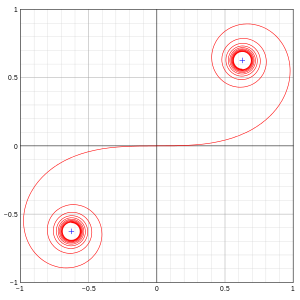
\includegraphics[width=.5\textwidth]{euler_spiral}
	\caption{A double-ended Euler spiral}
	\label{fig:euler_spiral}
\end{figure}

The racing line follows a segment of the Euler spiral that connects a starting point with an end point. This come close to minimizing the curvature, but does not completely reach the minimum. Also there are multiple segments that connect two points, so as, usually, the least curvature is wanted, the segment with the biggest radius is taken.

Most of these methods either need exact knowledge of the track or a simulation to work. This paper discusses possibilities to compare racing lines on an arbitrary track with no additional software other than a web browser.

\clearpage
	\section{Algorithm/Concept}
\label{sec:algorithm}
\graphicspath{{utils/}}
As this Bachelor Thesis tackles two problems, the algorithms can be divided into two categories as well.
The first category consists of racing line recording concepts and the second one of ways to compare these recordings.

\subsection{Recording}
\subsubsection{Visual Odometry}
\label{subsec:vo}
Visual Odometry (VO) is a concept that most camera-based robots use for navigation. It uses two consecutive camera frames to calculate the rotation and translation of the camera between them. The advantage over traditional tracking systems like GPS is, that it isn't dependent on any external sources, like satellites or radio towers, to determine the position of the object.

Also it is capable of much higher polling rates than most GPS receivers, which normally poll at 1 Hz, so they get 1 positional update per second. The potential speed of Visual Odometry is linked to the frame rate of the camera. That way, a camera that records at 30 frames per second enables Visual Odometry to estimate a position 30 times a second. 
The crude algorithm behind VO determines and stores recognizable features in one frame, using a feature detection algorithm.
At first we need two consecutive, rectified camera images. It is important that the images are rectified, because otherwise the edges of the image would be curved and produce wrong results.

Our solution uses the Harris corner detection method for determining features. Finding corners in an image is a very important prerequisite for the final position determination, because it allows us to calculate direction vector to another point. This other point being the same feature in the following camera frame, where the Harris detector is used, as well.

Having two sets of corners from either image we can track each feature from one frame to another. 
\begin{itemize}
    \item Lucas-Kanade?
    \item Jacobian?
\end{itemize}
Now that we have an end point to every (possible) starting point, we can construct a set of directional vectors.
Removing outliers (i.e. vectors that are much longer or go in a vastly different direction than most vectors) an approximation translation and rotation the camera conducted during the two frames can be calculated.

Outlier removal is an important stop, because otherwise external movements, like those of other cars on the track, might cause the algorithm to think the camera was moving in a different direction than it actually was.
To do that we used an iterative method called \textit{Random Sample Consensus} (RANSAC). 
The RANSAC algorithm works by taking a random subset of all the available data, in our case the vectors obtained by VO, and fitting a linear model with a specified neighborhood which contains this subset. All other vectors are then tested against this model and those who fit the model are considered part of the \textit{consensus set}.
If enough vectors lie within this model, it is considered as a viable candidate for a linear approximation. Optionally, the model can be re-evaluated using all vectors in the consensus set.

This sequence of events is repeated a fixed amount of times, each time producing a model which is rejected, because it contains too few inliers, or a refined model, if the model consists of more inliers than the best model so far.

If the taken path includes loops it is possible to optimize the result by using loop detection. If any features are re-detected at a later point in time and the current position is close to the position the features were re-detected, the path can be stretched in a way that it connects to the earlier path.
This can reduce errors that accumulated due to small estimation errors in the previous steps.

%%%%%%%%%%%%%%%%%%%%%%%%%%%%%%%%%%%%%%%%%%%%%%%%%%%%%%%%%%%%%%%%%%%%%%%%%
%TODO:
%\begin{itemize}
%  \item track features from one image to another (Lucas-Kanade-Method)
%  \item optimize result (Loop-Detection, Algorithm)
%\end{itemize}

\subsubsection{Lane Detection}
Lane Detection uses markings on a road to determine its lateral boundaries in relation to the recording camera. It is often used in autonomous driving and driving assistance systems, because the position of the car in between lane markings gives a lot of information about the direction the car is traveling. 
In our case, not only can we determine a traveling direction, but also the position on the lane.
By tracking the distance to the left and right lane, a deviation to the middle of the lane can be calculated. 
If the driven track is know or the camera is capable of determining a scale (e.g. by using a stereo camera), the deviation can even be expressed as a metric length, which is helpful for extracting additional information, like speed and acceleration, later on.


%TODO: Algorithms
\begin{itemize}
  \item possibility to improve recording results on known track
  \item possibility to determine accurate horizontal position on track
\end{itemize}

\subsubsection{Recording OBD2 Data}
\textit{Definition} OBD II (On-board diagnostics 2) is an interface which all cars build after 1996 in the USA or after 2003 in the EU, respectively, have to have built-in. It implements the SAE J1962 standard which provides standardized PIDs that return specific car-based sensor data, like the current speed, current motor revolution (rpm), throttle position and more.
A data request is possible about 10 times per second. This gives us a good basis for further detailed comparisons combined with the racing line recording.

\subsection{Comparing}
\subsubsection{Visual Comparison of Racing Line with help of sensor data}
A fairly simple, but effective way to find out where time is lost on the track is the visual comparison of racing lines from different drivers. The idea is to overlay the previously recorded lines over the race track. To actually determine at which point a driver was faster than the other one, we need an obvious optical representation of the speed at any given point on the track and the possibility to receive further information on demand.
In our system, the speed is represented by coloring in the racing line on a gradient scale reaching from green (standing still) to red (>250 km/h).
%TODO: Algorithm here
Besides speed data, different values, like acceleration, braking behavior or lap time, can be displayed in a similar fashion. That way the fastest line for a given corner can be determined and the slower driver can find out, why their line was inferior.

\begin{itemize}
  \item highlight relevant locations, like corners, showing detailed information about throttle and brake behavior and curvature through the corner
  \item fastest way through corner is trade-off between distance traveled and curvature, with low curvature allowing the driver to carry more speed to exit of the corner
\end{itemize}

\subsubsection{Mathematical Calculation of ideal line given a certain track}
Besides comparing two driver-generated racing lines, it is also possible to calculate a fast, almost ideal racing line.

\textit{Bézier Curves}
Bézier curves are a way to depict an entire race track, i.e. a curved path, with a set of control points, \{P\textsubscript{0}, P\textsubscript{1}, ..., P\textsubscript{n}\}. In this definition, n is the order of the curve. P\textsubscript{0} and P\textsubscript{n} stand for the beginning and the end point of the curve, respectively, while the intermediate points define the curvature of the curve and don't usually lie on it.

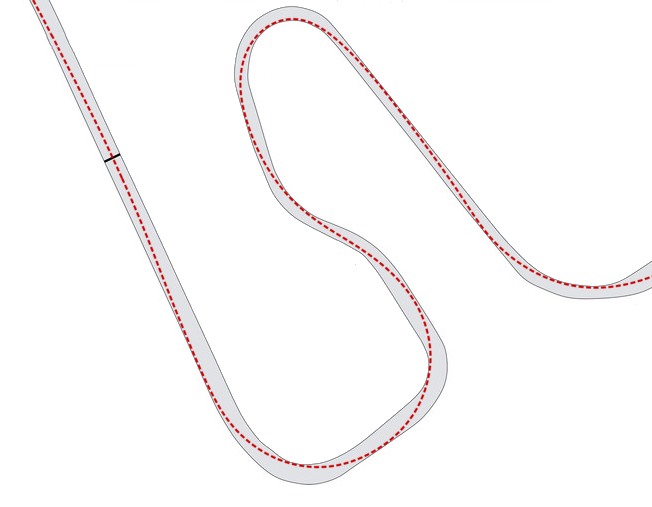
\includegraphics[width=\textwidth]{bezier_track}

As we want to get the line with the least curvature, the Bézier curve is capable of creating a fair approximation, especially suitable for racing beginners.


\subsubsection{Mathematical Comparison of two paths}
To gain additional and more detailed information about the driven racing line, it is helpful to get mathematical values for specific areas (e.g. the entry and exit angle of curves). This can tell a driver that their line was too shallow or too wide and provide the potential to improve.
For this technique we can use either racing line detection algorithm, even GPS. Every pair of consecutive points is turned into a vector, consisting of the distance between the points and the angle $\theta$ to the x-axis (the equator in case of GPS).
\begin{center}
$\Delta x = endPoint.x - startPoint.x$

$\Delta y = endPoint.y - startPoint.y$

$\overline{xy} = \sqrt{\Delta x² * \Delta y²}$

$\theta = \arctan(\frac{\Delta x}{\Delta y})$ 
\end{center}

To speed up subsequent calculations all consecutive vectors with the same $\theta$ can be combined into one vector by generating a new vector with the sum of the magnitude of the old ones. This indicates a straight where the individual sections aren't that interesting.
Now the angle of each section of a corner can be compared. Again, the coloring-approach may be used as a simple way to determine the angle at a glance.
\clearpage

	\section{Implementation}
\label{sec:implementation}

\subsection{Recording}
\subsubsection{Visual Odometry}
\subsubsection{OBD2 Data}

\subsection{Comparison}
\subsubsection{Google Maps}
\begin{itemize}
	\item calculate GPS coordinates from VO points
	\item Polyline Overlay
	\item hidden Polyline for calculations and hover function vs visible, colored Polyline	
\end{itemize}
	\section{Evaluation}
\label{sec:evaluation}

\subsection{Visual Odometry to record Racing Lines}
Visual Odometry has many theoretical advantages over GPS. The amount of data points received is a lot higher, as it produces 1 position per frame, which could realistically result in 30 - 60 positional updates per second, wheres GPS usually produces 1 point per second. This high amount of points makes a detailed comparison and analysis a lot easier, as curves appear mostly smooth instead of having only a couple of straight lines, as seen in figure \ref{fig:vo_gps_comp}.

\begin{figure}[!ht]
	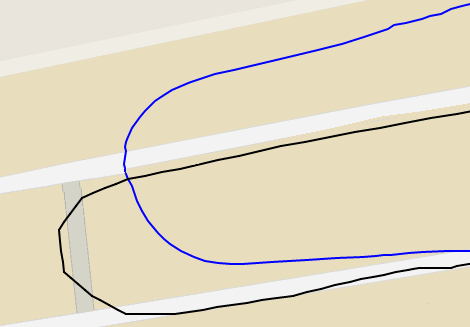
\includegraphics[width=\textwidth]{VO_corner_comp}
	\caption{Visual Odometry (blue) produces much smoother curves than GPS (black), but can be erroneous}
	\label{fig:vo_gps_comp}
\end{figure}

Consequently, VO is capable of detecting very small movements. A racing car driving at 100 km/h travels ~28 meters forward every second. The lateral movement, i.e. driving from one side of the track to the other or through corners, is much slower. So, assuming a driver takes 2 seconds to cross a 10 m wide track, we would get one positional update every 17 cm at 30 frames per second. 

Obviously, this is 30 times better than GPS because of the higher speed alone, but also the GPS standard (NMEA 0183) is only accurate to $\frac{1}{60 000}$ of a degree. The distance between two degrees of latitude is 110 km, the distance between two meridians at 51° (position of Berlin) 70 km. That means the accuracy in North-South direction is 1.8 m and in East-West direction 1.2 m. If the Region of Interest (ROI) of our camera image has a real-world width of 30 m and the recording has Full-HD resolution, the accuracy of VO would be 3 cm.
Another advantage of Visual Odometry is that it doesn't rely on external sources, like satellites, and is in general mostly independent of the area it is used. After all, even the Mars Rovers used this algorithm to navigate. Especially in forests, rural areas and tunnels, GPS is either inaccurate or not usable at all. The camera-based approach still works when GPS fails.
So all in all, VO is able of extracting a very detailed depiction of the racing line, even in remote areas. However, the algorithms used are fairly expensive.
A mobile-range computer (like the NVidia Jetson TX1) can achieve an average frame rate of about 8 frames per second at a resolution of 672 x 376 px. This is in theory still better than GPS, but it is an average value, potentially becoming a lot slower in feature-dense areas, like forests, and especially corners. The reason VO slows down in corners is, that rather than tracking already existent features points it has to search new points much more frequently than on straights, because the scenery changes much quicker.
Additionally, VO can only determine a relative difference to the last calculated position. This means, that potential errors, like too shallow corner angles, will result in faulty results throughout the entire path. This can also be seen in figure \ref{fig:vo_gps_comp}. The incoming and outgoing straights should be close to parallel, but the VO image detected them at an angle. If this turn would be repeated, the error would cause the line to not be consistently at the same position every time, without further processing.

Most of these limitations are caused by the desire to achieve a real-time capable solution. If speed is not an issue, the error rate can be reduced a lot. So, for a quick draft it is sensible to use GPS, however if it is possible to record the drive and sufficient to analyze it at a later time, VO creates more accurate results. 

\subsection{Usefulness of Racing Line Comparison}
Professional drivers can usually handle their cars very well, however only the best drivers have the feeling and intuition for the fastest racing line. Studies showed, that techniques like trail braking, which means that the driver breaks into the corner, until they reached the apex, in contrast to doing all the braking on the straight, improve lap times by up to 5\%, which makes a difference of 4 seconds on an 80 second lap \cite{gustafsson08}. Being able to compare braking points between drivers and a calculated optimal line can therefore make the difference between winning and losing.\\
In addition to the possibility of improving ones lap time, especially amateur and intermediate drivers can experience an even more competitive race. Now the award for driving fast is not only a fast time, but also the visual confirmation, that shows where and why a driver was the best and it increases the challenge, as weaker drivers can improve faster.\\
A gamification element, like a level that reflects the drivers skill, could be introduced to further expand this criterion.

\clearpage

	\section{Future Work}
\label{sec:future_work}

\subsection{Open Research Questions}
\subsubsection{Real Time Capabilities}
\subsubsection{Increasing Accuracy}

\subsection{Extensions}
\subsubsection{Gamification}
So far drivers already have a simple and accessible way of comparing each other, however our method only provides a direct relation between two drivers. Unless a driver looks at all other drivers racing lines, they can't certainly asses if they drove a particularly fast lap or if the opponent was just slow in general.\\
Thats why a form of gamification could be implemented. Based on different factors, like cornering, control and boldness, a score could be determined that assigns a level to a driver. That way drivers could compare, even if they didn't drive on the same track and races could include drivers of similar skill levels to make them as intense as possible.

\subsubsection{Real-Time Comparison}
Currently, the recording of the racing line can not be achieved completely in real-time with hardware that is power-conscious enough to run with the power provided by a cars battery, as the most powerful hardware that can be considered to fulfill this requirement is the NVidia Jetson TX1, which we used. However, current implementations of Visual Odometry tend to not use the full capabilities of the device, namely they only run on the CPU, while the GPU is running idle. If, either using more powerful hardware or very specifically optimized algorithms, VO could be implemented to run in real-time, i.e. at 30-60 frames per second, this would make it possible to determine an exact location of the car at any point of the race, without the delay of sending the video data to a central, powerful processing unit or the inaccuracy of having to skip frames.\\
The position could then be transmitted directly to other cars and their drivers to inform them about how they compete in relation to all other drivers. Such an overview could even be shown in a heads-up display directly on the windscreen or, in order to not disturb the driver too much, by informing the team manager of the driver, who can then tell the driver.\\
The advantage of this process is, that no expensive measurement equipment and, especially, no external dependencies (apart from the communication between the cars) are needed. So it could be used anywhere.

\clearpage
	\section{Conclusion}
\label{sec:conclusion}
In order to develop an accessible racing driver analysis we explored a variety of methods to record and assess the driving behavior of racers. As our system should have as little external dependencies as possible, we looked for methods to do all of the analysis inside the car, which is why camera-based methods were used to record the racing line and race track. 

Additionally, we used the cars on-board sensor data to obtain further information about the driving and consequently enable us to answer complex questions, like the ideal braking and acceleration points on the track.

This made it possible to compare two drivers and discover their strengths and weaknesses and how to tackle them to become a better racing driver. Alternatively, an ideal racing line could be calculated, even without prior knowledge of the track with the help of lane detection. This could help even professional drivers improve and achieve best times.

Further improvements can be made through the addition of a gamification system, that gives a level to a driver based on their skill. Also with the help of a more optimized implementation a real-time comparison could be achieved, that could tell a driver at any time how they compare to another driver, e.g. displaying it at a heads-up display directly on the screen.
\clearpage

	%%%%%%%%
	
	%%% BIBLIOGRAPHY
	%\bibliographystyle{babunsrt3-fl}
	\addcontentsline{toc}{section}{Bibliography}
	\bibliographystyle{ieeetr}
	\bibliography{projektbib}
	\clearpage	
	
	%\appendix
\section{Appendix}
\label{sec:appendix}

Lorem ipsum dolor sit amet, consectetur adipiscing elit. In erat mauris, faucibus quis pharetra sit amet, pretium ac libero. Etiam vehicula eleifend bibendum. Morbi gravida metus ut sapien condimentum sodales mollis augue sodales. Vestibulum quis quam at sem placerat aliquet. Curabitur a felis at sapien ullamcorper fermentum. Mauris molestie arcu et lectus iaculis sit amet eleifend eros posuere. Fusce nec porta orci.

Integer vitae neque odio, a sollicitudin lorem. Aenean orci mauris, tristique luctus fermentum eu, feugiat vel massa. Fusce sem sem, egestas nec vulputate vel, pretium sit amet mi. Fusce ut nisl id risus facilisis euismod. Curabitur et elementum purus. Duis tincidunt fringilla eleifend. Morbi id lorem eu ante adipiscing feugiat. Sed congue erat in enim eleifend dignissim at in nisl. Donec tortor mauris, mollis vel pretium vitae, lacinia nec sapien. Donec erat neque, ullamcorper tincidunt iaculis sit amet, pharetra bibendum ipsum. Nunc mattis risus ac ante consequat nec pulvinar neque molestie. Etiam interdum nunc at metus lacinia non varius erat dignissim. Integer elementum, felis id facilisis vulputate, ipsum tellus venenatis dui, at blandit nibh massa in dolor. Cras a ultricies sapien. Vivamus adipiscing feugiat pharetra.
	
	
\end{document}
